\chapter{Einleitung}

Softwarequalitätsmanagement (SQM) ist ein entscheidender Aspekt bei der Entwicklung und Implementierung von Softwarelösungen, 
um sicherzustellen, dass sie effizient, sicher und zuverlässig sind. In dieser Hausarbeit werden wir uns mit dem Vorgehen 
hinsichtlich SQM auseinandersetzen und Optimierungen entwerfen, indem wir ein praktisches Fallbeispiel untersuchen. 
Unser Anwendungsbeispiel ist die Integration einer Recommendation Engine (RE) in eine Lernplattform mit Gamification 
auf dem Hyperscaler Amazon Web Services (AWS). Dieses Beispiel dient dazu, sowohl theoretisches Wissen als auch praktische 
Anwendungsfähigkeiten in Bezug auf SQM nachzuweisen.

Bei meiner Firma, der SAP, gibt es intern eine Lernplattform die Gamification nutzt, um SAP-interne Prozesse 
spielerisch den Kollegen zu vermitteln. Diese Plattform heißt \textit{Digital Heroes}. 
Bisher können die Kollegen die Lernplattform nach konkreten Inhalten durchsuchen. 
Außerdem können die Moderatoren bestimmte Inhalte auf der Startseite featuren. Es gibt jedoch keine 
personalisierten Empfehlungen von Lerninhalten für die Nutzer der Plattform. 
Durch das Einführen einer in-house RE soll sich das nun ändern und damit den Prozess für Nutzer an neue Inhalte 
zu gelangen verbessern.  \\
Das Problem beim Integrieren der RE ist allerdings, dass die bisherige Software dafür angepasst 
und vorbereitet werden muss. Insbesondere arbeitet die RE auf stark-assoziierten Daten, 
was viele sehr aufwendige Joins in der derzeitig genutzten relationalen Datenbank nötig macht, 
was sehr ressourcenintensiv ist.  
Ziel des hier genutzten Anwendungsbeispiels ist es also die RE in die bestehende Software so zu integrieren, 
dass andere Systemteile nicht beeinträchtigt werden. 

Um dieses Ziel zu erreichen, soll das erworbene Wissen aus der Softwarequalität-Vorlesung genutzt werden, 
um das Problem kritisch zu analysieren und zu optimieren. 
Dafür wird zunächst die Ausgangssituation des aktuellen Prozesses untersucht, 
daraufhin wird betrachtet, warum die RE eingeführt wird und warum das bestimmte Anpassungen an der 
bestehenden Software nötig macht. Darauf aufbauend wird beschrieben, wie dadurch der bestehende 
Prozess verbessert werden kann. Weiter wird analysiert, welche Optimierungsmöglichkeiten aus der Sicht 
der SQM es hierfür gibt. Anschließend wird betrachtet, wie der Prozess nach der Optimierung aussieht. 
Schließlich werden in einer Zusammenfassung die grundlegenden Erkenntnisse der Arbeit nochmals bündig dargelegt.

\chapter{Derzeitiger Prozess}

Die gamifizierte Lernplattform namens Digital-Heroes (DH) kann derzeit nach Lerninhalten durchsucht werden 
und es werden \textit{Featured Missions} angezeigt.
Bei dem Durchsuchen nach Lerninhalten kann derzeit eine Volltextsuche verwendet werden. 
Es kann zudem nach groben Kategorien geordnet werden. 
Die Featured Missions, die in \autoref{fig:dh-website} abgebildet sind, 
werden durch das Moderatorenteam ausgewählt -- es steht kein automatischer 
Algorithmus dahinter.

\begin{figure}
	\centering
	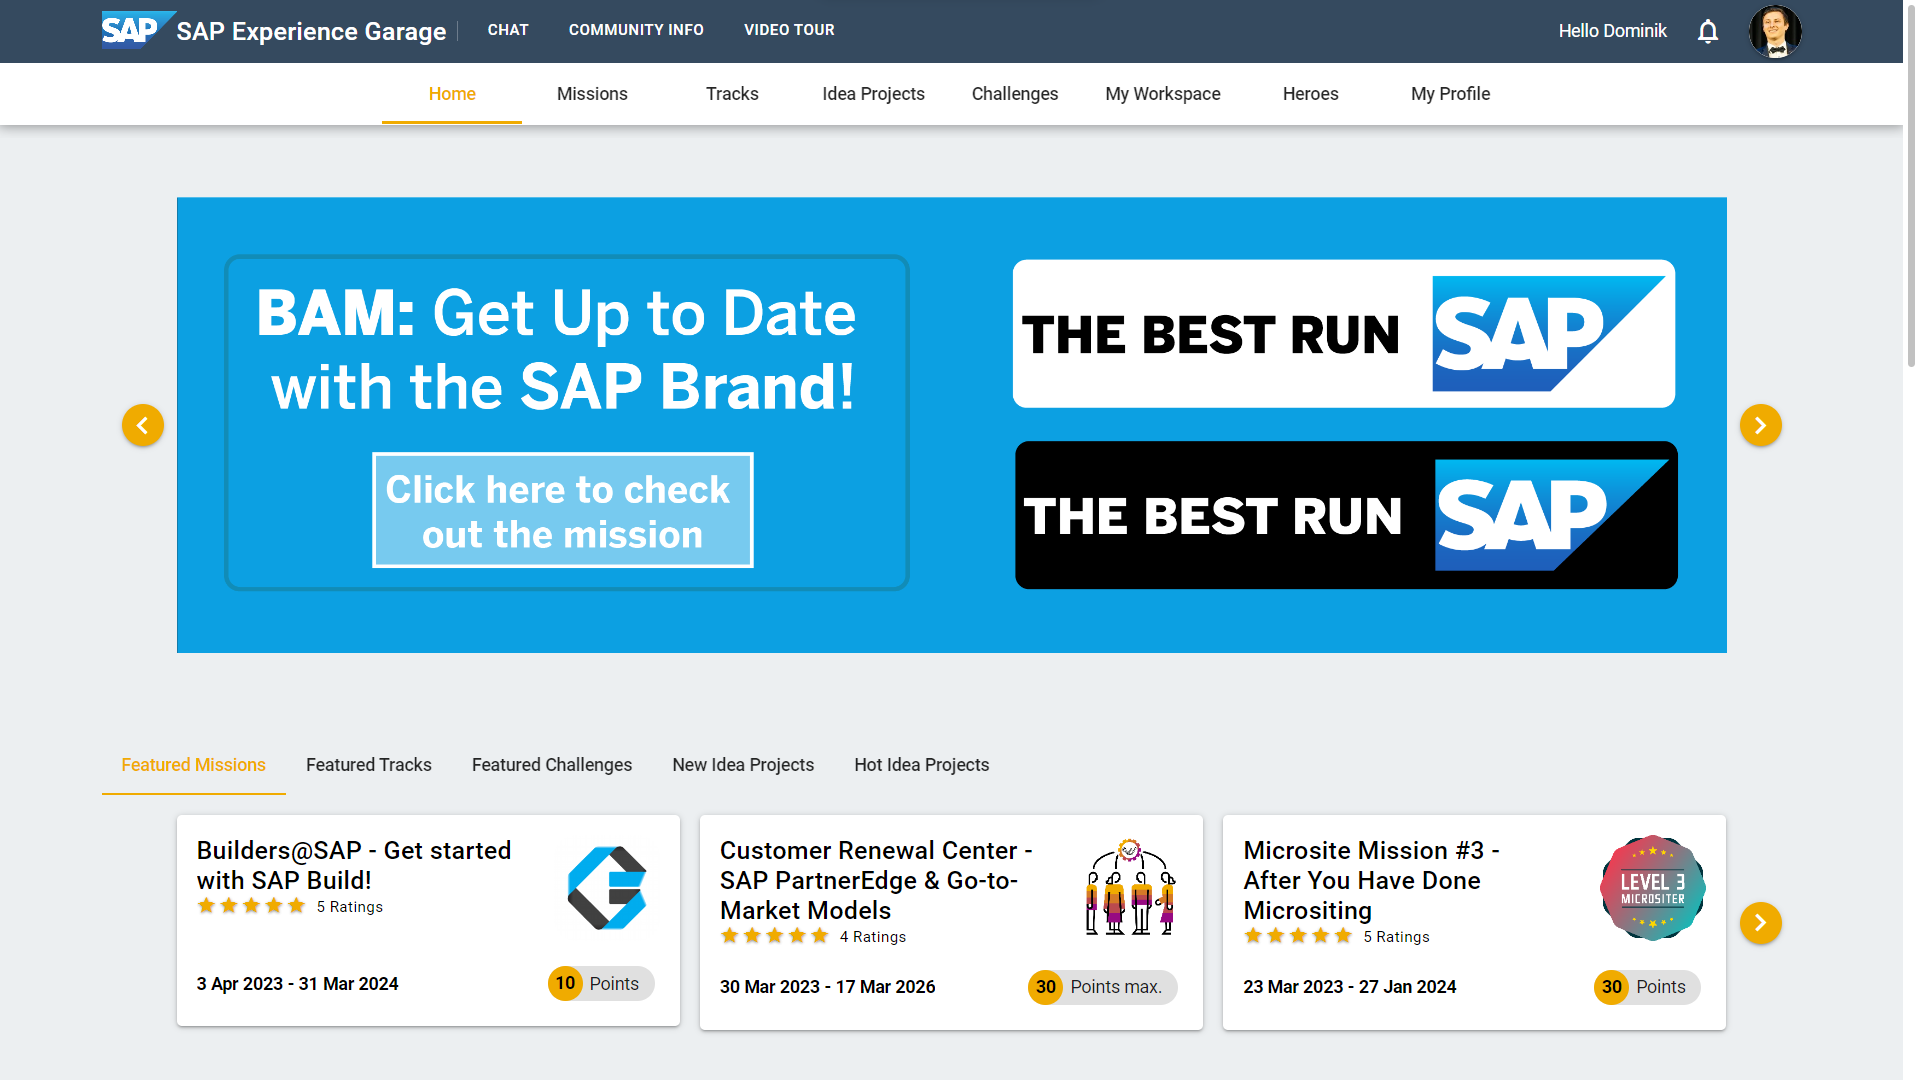
\includegraphics[width=1.\textwidth]{Bilder/dh-website.png} 
	\caption{Die Abbildung zeigt die Landing-Page der Digital-Heroes-Lernplattform. 
    Insbesondere lässt sich der Tab der \textit{Featured Missions} erkennen.}
	\label{fig:dh-website}
\end{figure} 

Der Prozess der Auswahl der Featured Missions läuft wie folgt ab: 
\begin{enumerate}
    \item Ein Nutzer oder Moderator erstellt einen neuen Lerninhalt (Mission).
    \item Der neue Inhalt wird von einem Mitglied des Moderatorenteams überprüft (Review), 
    bevor diese Mission veröffentlicht wird.
    \item Ein mal die Woche stimmt sich das Moderatorenteam ab und entscheidet 
    sich für die besten Missionen, die diese Woche erstellt wurden, welche 
    dann in der nächsten Woche gefeatured werden. 
\end{enumerate}
Dieser Prozess und das Fehlen eines automatischen Vorschlagssystems führt 
zu Frustration sowohl aufseiten der Nutzer als auch aufseiten der Moderatoren. 
Die Nutzer würden gerne mehrmals die Woche neue Vorschläge 
(derzeitig die Featured Missions) bekommen und für sie relevante 
Themen direkt vorgeschlagen bekommen, ohne danach explizit suchen zu müssen. \\
Für die Moderatoren ist es dagegen ein großer Arbeitsaufwand 
sich für die Featured Missions zu entscheiden, insbesondere 
ist dabei die Abstimmung mit den anderen Moderatoren zeitaufwendig 
als weiteres Meeting. 

\chapter{Warum eine Recommendation Engine (RE) und was wird dafür nötig?}

Um den Prozess aus dem vorangegangenen Kapitel zu verbessern, 
muss eine automatische Lösung eingebaut werden. \\
In einer benachbarten Abteilung wird eine experimentelle Recommendation Engine (RE) 
namens DANOS entwickelt. Dementsprechend war mein Vorschlag, 
diese für Digital Heroes zu verwenden. Für die entwickelnde Abteilung 
hat dies auch den Vorteil, dass diese frühzeitig schon mit einem praktischen Use-Case 
und einer Success-Story werben können. Für die Nutzer von Digital Heroes 
ermöglicht es, dass sie beliebig viele, genau auf sie zugeschnittene Empfehlungen 
von Lerninhalten bekommen können. Die Moderatoren sparen sich den Aufwand 
der Ermittlung der Featured Missions, da diese ersetzt werden können durch die 
personalisierten Vorgaben. 

Damit die RE integriert werden kann, wird allerdings ein anderer persistenter Speicher nötig.
Grob beschrieben erstellt die RE ihre Empfehlungen für Nutzer A über 
die Präferenzen und bereits absolvierten Missionen von Nutzer B, wenn Nutzer B \textit{ähnlich}
zu Nutzer A ist. Das heißt, um den Rechenaufwand zu verringern, 
soll ein mal berechnet werden, welche Nutzer sich ähnlich sind und die 
Ergebnisse sollen gespeichert werden. Bisher sind alle Inhalte der Lernplattform 
in einer relationalen Datenbank abgelegt. Die RE muss für das Einordnen 
von neuen Inhalten und Nutzern die Ähnlichkeitsbeziehung 
über mehrere Nutzer verfolgen. In einer relationalen Datenbank, 
in dem Nutzer paarweise mit einem Ähnlichkeitsscore abgelegt sind, 
erfordert das Verfolgen der Ähnlichkeit über mehrere Nutzer Datenbankjoins 
derselben Tabelle abhängig von der Länge der Ähnlichkeitskette $n$. 
Bei $m$ Nutzern würde eine Abfrage der Ähnlichkeitskette der Länge $n$ 
eine Tabelle mit $m^n$ Einträgen generieren. Bei bspw. $m = 10000$ und $n=3$ 
bereits $m^n = 10000^3 = 10^{12} = 1~Billion$ Einträge. 

\begin{figure}
	\centering
	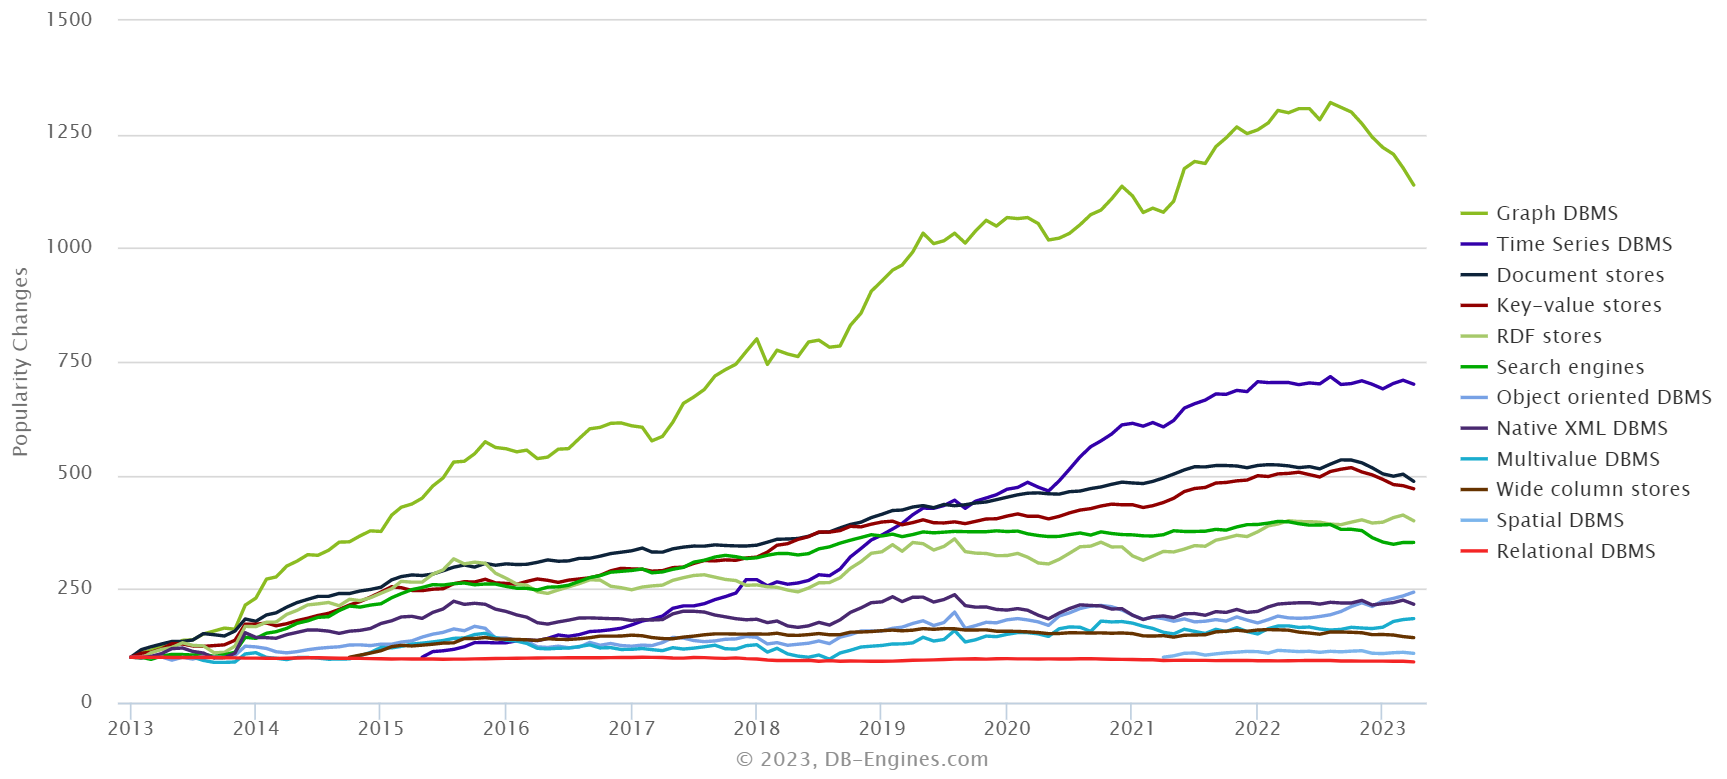
\includegraphics[width=1.\textwidth]{Bilder/graph-db-rise-popularity.png} 
	\caption{Anstieg der Popularität verschiedener Datenbankmodelle. (Entnommen aus \cite{db-ranking}.)}
	\label{fig:db-ranking}
\end{figure} 